\chapter{Расчет режимов спроектированной сети в ПВК RastrWin3}
\label{cha:растр_вин}

\counterwithin{figure}{section}

\section{Моделирование и расчет режима наибольших нагрузок}

Параметры узлов для режимов НБ и П/АВ приведены на рис. \ref{fig:узлы_нб}, параметры ветвей для режимов НБ и П/АВ приведены на рис. \ref{fig:ветви_нб}.

\begin{figure}[H]
	\centering
	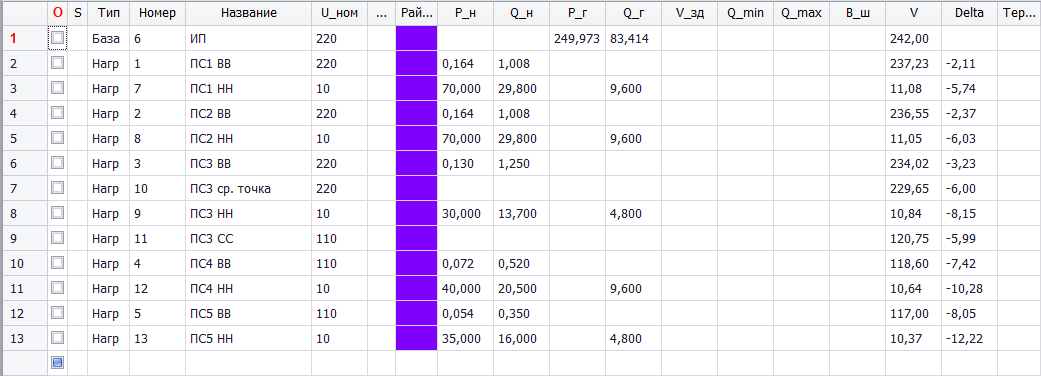
\includegraphics[width=1\textwidth]{inc/img/режим_нб_узлы}
	\caption{Исходные данные по узлам в режиме НБ и П/АВ и результаты расчёта режима НБ во вкладке «Узлы» без регулирования напряжений}
	\label{fig:узлы_нб}
\end{figure}

\begin{figure}[H]
	\centering
	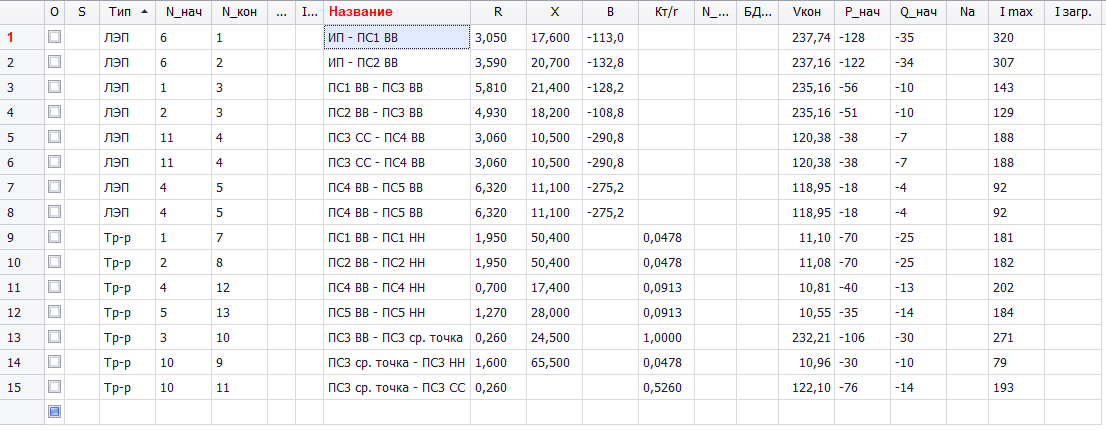
\includegraphics[width=1\textwidth]{inc/img/режим_нб_ветви}
	\caption{Исходные данные по узлам в режиме НБ и П/АВ и результаты расчета режима НБ во вкладке «Ветви» без регулирования напряжений}
	\label{fig:ветви_нб}
\end{figure}

Параметры регулировочных устройств приведены на рис \ref{fig:анцапфы}.

\begin{figure}[H]
	\centering
	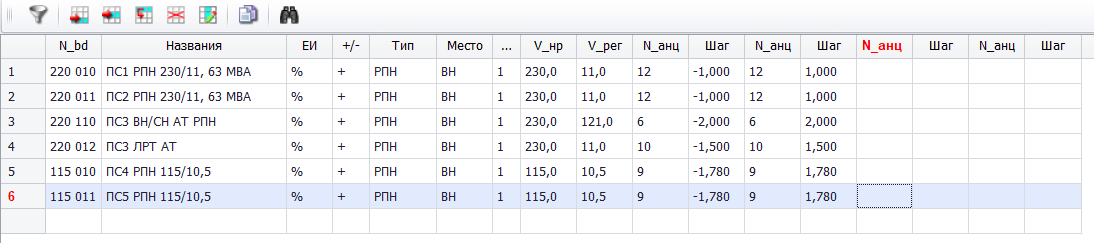
\includegraphics[width=1\textwidth]{inc/img/режим_нб_рпн}
	\caption{Параметры регулировочный устройств}
	\label{fig:анцапфы}
\end{figure}

Результаты регулировки напряжений в режиме НБ приведены на рис. \ref{fig:узлы_нб_отрег}, \ref{fig:ветви_нб_отрег}.

\begin{figure}[H]
	\centering
	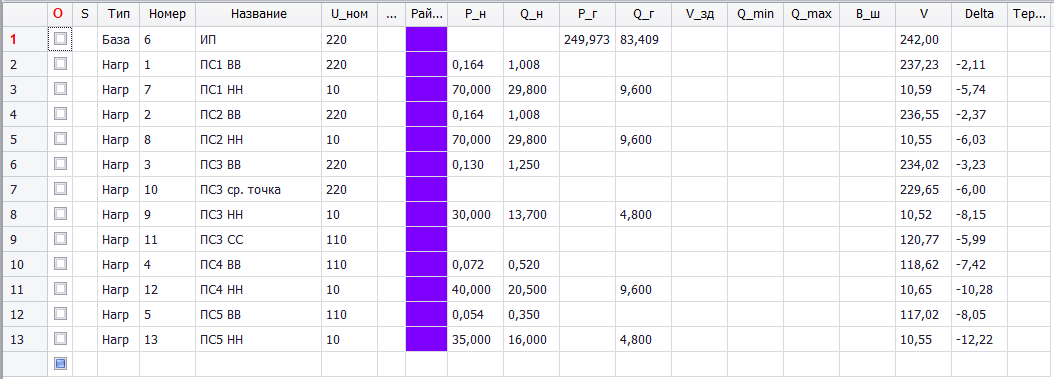
\includegraphics[width=1\textwidth]{inc/img/режим_нб_узлы_отрег}
	\caption{Результаты расчёта режима НБ после регулирования напряжения во вкладке «Узлы»}
	\label{fig:узлы_нб_отрег}
\end{figure}

\begin{figure}[H]
	\centering
	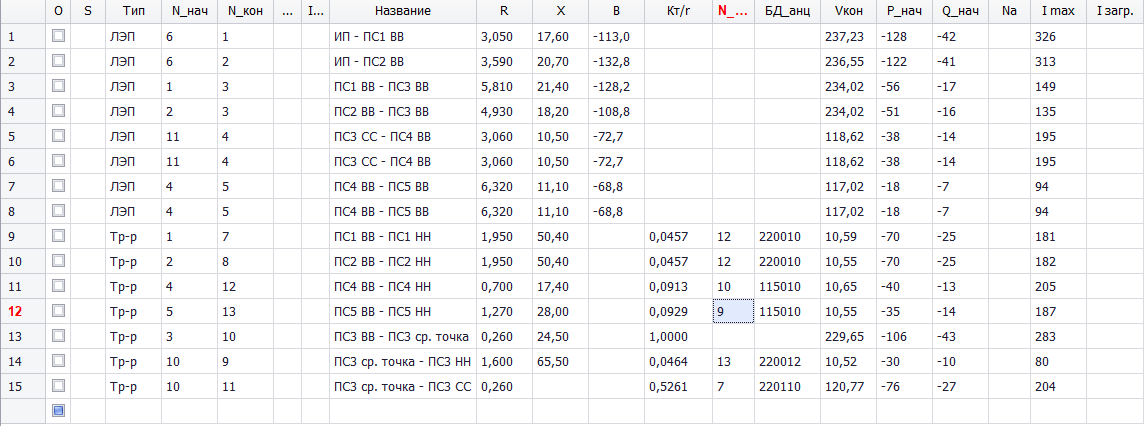
\includegraphics[width=0.95\textwidth]{inc/img/режим_нб_ветви_отрег}
	\caption{Результаты расчёта режима НБ после регулирования напряжения во вкладке «Ветви»}
	\label{fig:ветви_нб_отрег}
\end{figure}

\section{Моделирование и расчет режима наименьший нагрузок}

Параметры узлов для режима НМ приведены на рис. \ref{fig:режим_нм_узлы}, параметры ветвей для режима НМ приведены на рис. \ref{fig:режим_нм_ветви}.

\begin{figure}[H]
	\centering
	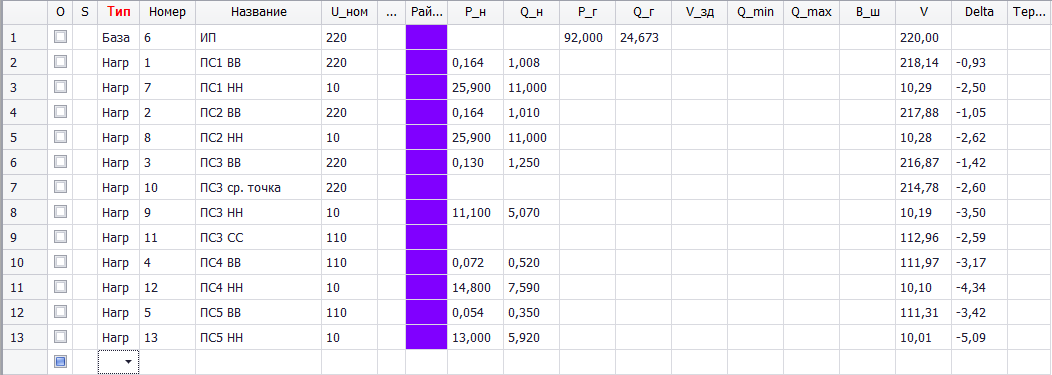
\includegraphics[width=1\textwidth]{inc/img/режим_нм_узлы}
	\caption{Исходные данные по узлам и результаты расчёта режима НМ во вкладке «Узлы» без регулирования напряжений}
	\label{fig:режим_нм_узлы}
\end{figure}

\begin{figure}[H]
	\centering
	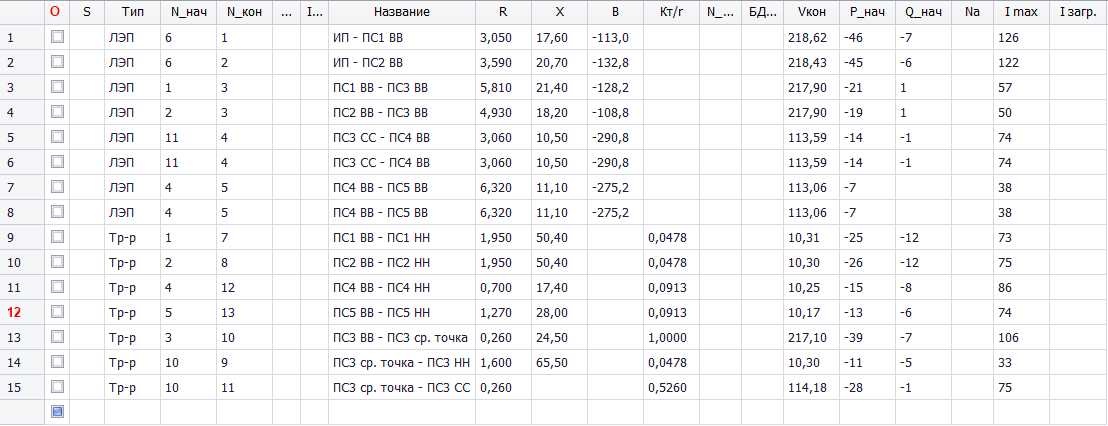
\includegraphics[width=1\textwidth]{inc/img/режим_нм_ветви}
	\caption{Исходные данные по ветвям и результаты расчета режима НМ во вкладке «Ветви» без регулирования напряжений}
	\label{fig:режим_нм_ветви}
\end{figure}

Результаты регулировки напряжений в режиме НМ приведены на рис. \ref{fig:режим_нм_узлы_отрег}, \ref{fig:режим_нм_ветви_отрег}.

\begin{figure}[H]
	\centering
	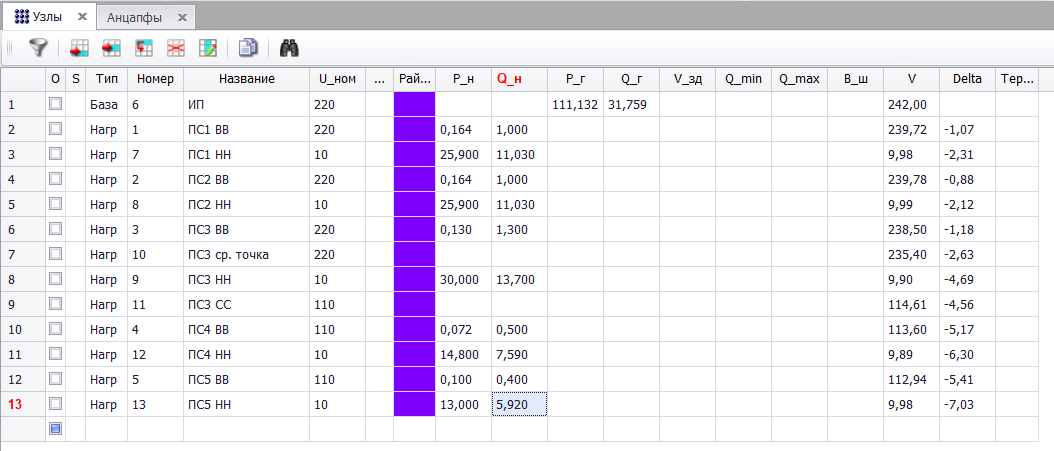
\includegraphics[width=1\textwidth]{inc/img/режим_нм_узлы_отрег}
	\caption{Результаты расчёта режима НМ во вкладке «Узлы» после регулирования напряжений}
	\label{fig:режим_нм_узлы_отрег}
\end{figure}

\begin{figure}[H]
	\centering
	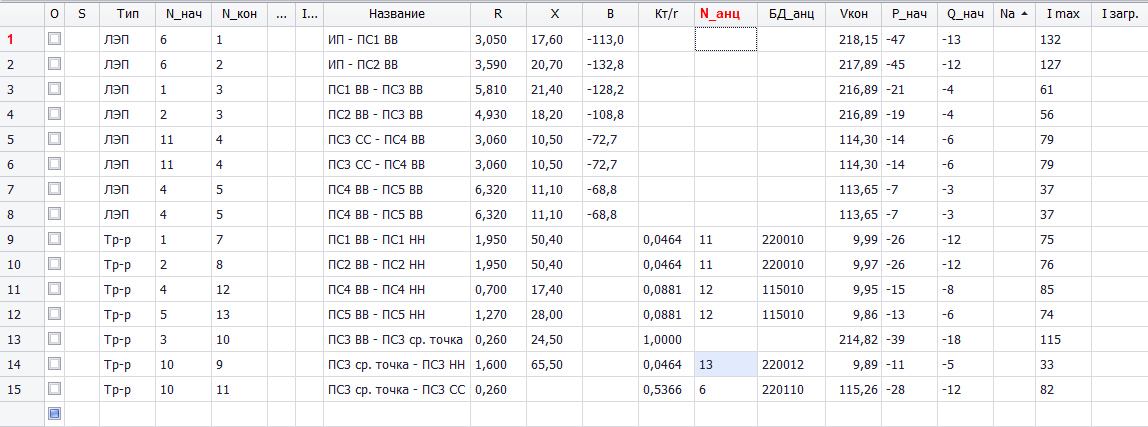
\includegraphics[width=1\textwidth]{inc/img/режим_нм_ветви_отрег}
	\caption{Результаты расчёта режима НМ во вкладке «Ветви» после регулирования напряжений}
	\label{fig:режим_нм_ветви_отрег}
\end{figure}

\section{Моделирование и расчёт послеаварийных режимов}

\subsection{Моделирование и расчет послеаварийного режима в сети 220 кВ}

Рассматривается послеаварийный режим в сети 220 кВ, при котором происходит отключение наиболее загруженного головного участка К-1 (см. значения токов на рис. \ref{fig:ветви_нб_отрег}).

Параметры узлов для П/АВ режима в кольцевой сети 220 кВ приведены на рис. \ref{fig:п/ав_в_сети_220_кв_узлы}, параметры ветвей для П/АВ режима в сети 220 кВ приведены на рис. \ref{fig:п/ав_в_сети_220_кв_ветви}.

\begin{figure}[H]
	\centering
	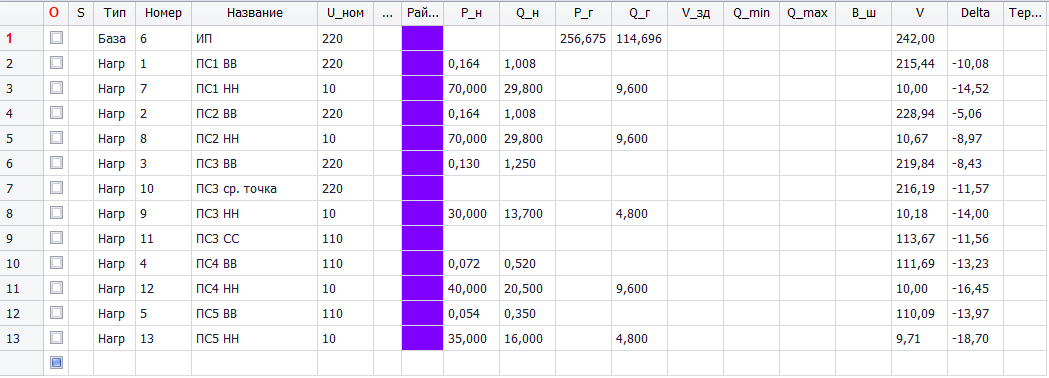
\includegraphics[width=1\textwidth]{inc/img/п_ав_220_кв_узлы}
	\caption{Результаты расчета П/АВ режима в сети 220 кВ при отключении линии К1 во вкладке «Узлы» без регулирования напряжений}
	\label{fig:п/ав_в_сети_220_кв_узлы}
\end{figure}

\begin{figure}[H]
	\centering
	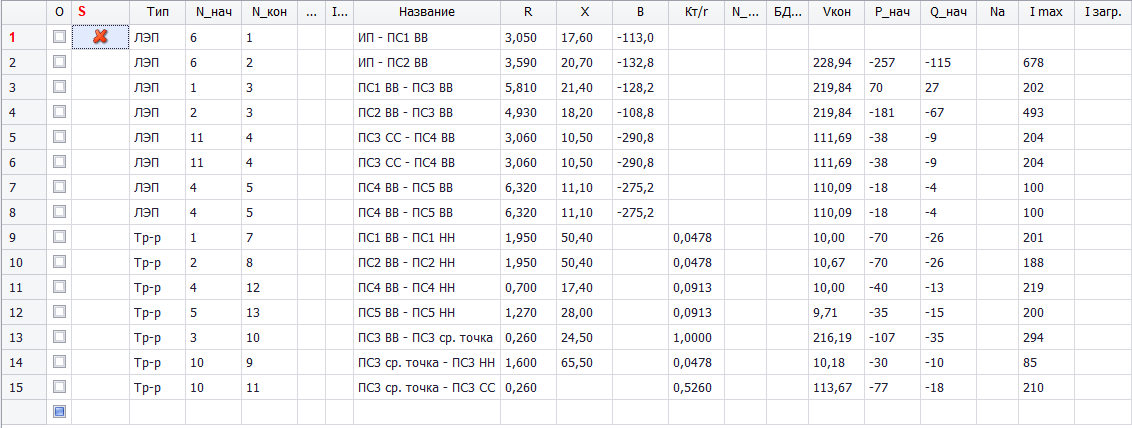
\includegraphics[width=1\textwidth]{inc/img/п_ав_220_кв_ветви}
	\caption{Результаты расчета П/АВ режима в сети 220 кВ при отключении линии К1 во вкладке «Ветви» без регулирования напряжений}
	\label{fig:п/ав_в_сети_220_кв_ветви}
\end{figure}

Результаты регулировки напряжений в режиме П/АВ в сети 220 кВ приведены на рис. \ref{fig:п/ав_в_сети_220_кв_узлы_отрег}, рис. \ref{fig:п/ав_в_сети_220_кв_ветви_отрег}.

\begin{figure}[H]
	\centering
	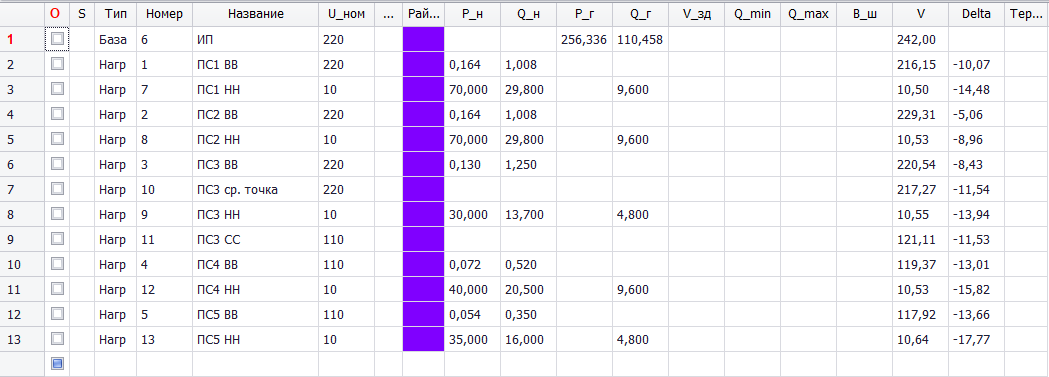
\includegraphics[width=1\textwidth]{inc/img/п_ав_220_кв_узлы_отрег}
	\caption{Регулирование напряжения на шинах НН и СН в П/АВ режиме в сети 220 кВ во вкладке «Узлы»}
	\label{fig:п/ав_в_сети_220_кв_узлы_отрег}
\end{figure}

\begin{figure}[H]
	\centering
	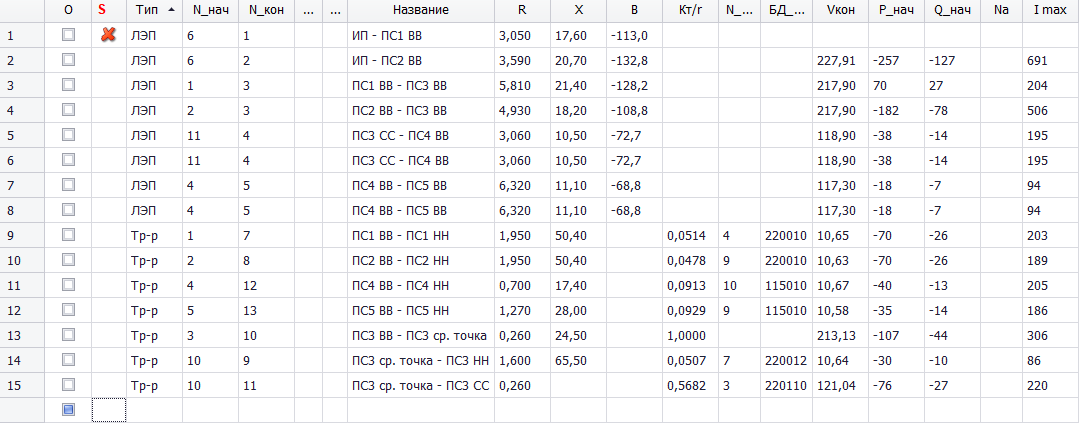
\includegraphics[width=1\textwidth]{inc/img/п_ав_220_кв_ветви_отрег}
	\caption{Регулирование напряжения на шинах НН и СН в П/АВ режиме в сети 220 кВ во вкладке «Ветви»}
	\label{fig:п/ав_в_сети_220_кв_ветви_отрег}
\end{figure}

\subsection{Моделирование и расчет послеаварийного режима в сети 110 кВ}

Рассматривается послеаварийный режим в сети 110 кВ, при котором происходит отключение одной цепи двухцепной линии 3-4.

Параметры узлов для П/АВ режима в сети 110 кВ приведены на рис. \ref{fig:п/ав_в_сети_110_кв_узлы}, параметры ветвей для П/АВ режима в сети 110 кВ приведены на рис. \ref{fig:п/ав_в_сети_110_кв_ветви}.

\begin{figure}[H]
	\centering
	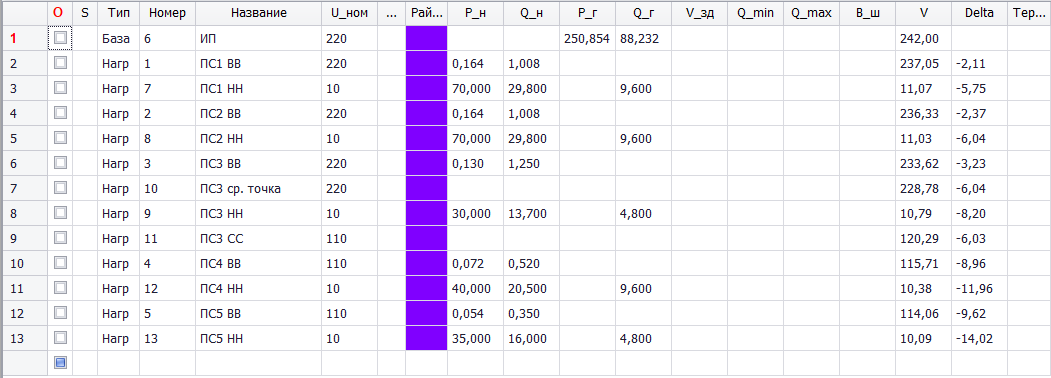
\includegraphics[width=1\textwidth]{inc/img/п_ав_110_кв_узлы}
	\caption{Результаты расчета после отключения наиболее нагруженного головного участка 34 для моделирования П/АВ режима в сети 110 кВ во вкладке «Узлы» без регулирования напряжений}
	\label{fig:п/ав_в_сети_110_кв_узлы}
\end{figure}

\begin{figure}[H]
	\centering
	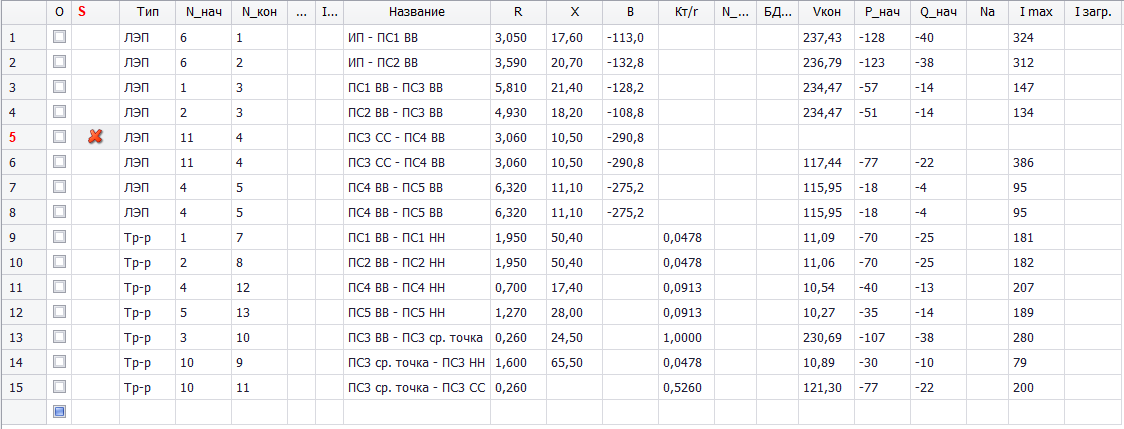
\includegraphics[width=1\textwidth]{inc/img/п_ав_110_кв_ветви}
	\caption{Результаты расчета после отключения наиболее нагруженного головного участка 34 для моделирования П/АВ режима в сети 110 кВ во вкладке «Ветви» без регулирования напряжений}
	\label{fig:п/ав_в_сети_110_кв_ветви}
\end{figure}

Результаты регулировки напряжений в П/АВ режиме в сети 110 кВ приведены на рис. \ref{fig:п/ав_в_сети_110_кв_узлы_отрег}, рис. \ref{fig:п/ав_в_сети_110_кв_ветви_отрег}.

\begin{figure}[H]
	\centering
	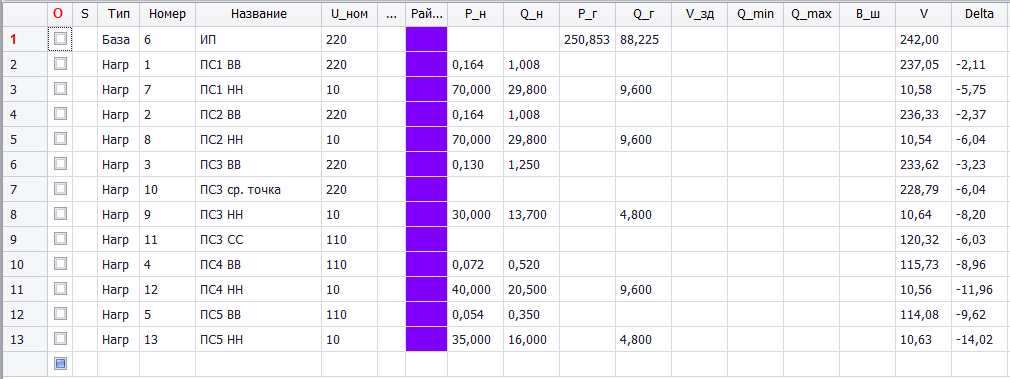
\includegraphics[width=1\textwidth]{inc/img/п_ав_110_кв_узлы_отрег}
	\caption{Результаты регулирования напряжения на шинах НН и СН в П/АВ режиме в сети 110 кВ при отключении наиболее нагруженного головного участка 34 во вкладке «Узлы»}
	\label{fig:п/ав_в_сети_110_кв_узлы_отрег}
\end{figure}

\begin{figure}[H]
	\centering
	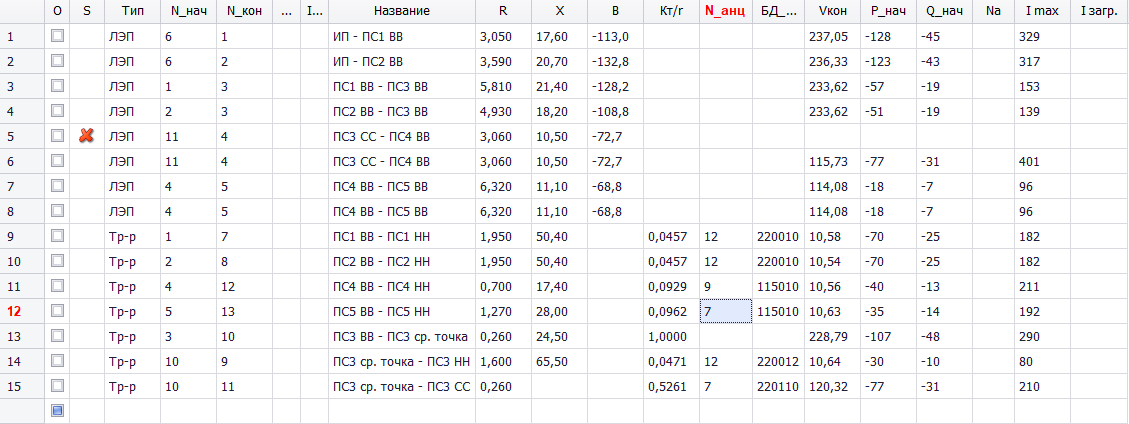
\includegraphics[width=1\textwidth]{inc/img/п_ав_110_кв_ветви_отрег}
	\caption{Результаты регулирования напряжения на шинах НН и СН в П/АВ режиме в сети 110 кВ при отключении наиболее нагруженного головного участка 34 во вкладке «Ветви»}
	\label{fig:п/ав_в_сети_110_кв_ветви_отрег}
\end{figure}